\section{Empirical Evaluation}
\label{sec:exp}

We evaluate our $\dfw(K)$ scheduler empirically by comparing its
sequentialization with an analogously implemented sequentialization of Emmi et
al.'s $\df(K)$ scheduler~\cite{conf/popl/EmmiQR11}; we have implemented
both sequentializations in the {\tt c2s}
tool\footnote{\url{https://github.com/michael-emmi/c2s}}. Since the
$\df(K)$ scheduler does not interpret \lstinline{wait} statements, we
pre-process each program given to the $\df(K)$-based sequentialization
with the translation of Figure~\ref{fig:tr:wait}, which outputs an equivalent
program without \lstinline{wait} statements. Essentially, this program keeps
track of whether each task has finished using the global \lstinline{result}
variable; the translation of each \lstinline{wait} statement for a task cannot
proceed until its task has completed.

\begin{figure}[t]
  \lstset{language=program}
  \lstset{basicstyle=\ttfamily\scriptsize}
  \begin{lstlisting}
    // new global declarations
    var result[int]: $T$;
    var uniqueId: int

    // translation of proc $p$(l: $T$) $s$
    proc p(l: $T$, self: int) $s$

    // translation of proc main() $s$
    proc main()
    result := [$\nil$, $\nil$, ..];
    uniqueId := 0;
    $s$

    // translation of call x := p e
    call x := p (e,0)

    // translation of return e
    result[self] := e;
    return e

    // translation of async t := p e
    t := ++uniqueId;
    async p(e,t)

    // translation of x := wait t
    x := result[t];
    assume x != $\nil$
  \end{lstlisting}

  \caption{A preprocessing step for the $\df(K)$ sequentialization to
    remove wait statements.}
  \label{fig:tr:wait}
\end{figure}

All of our experiments are carried out by applying a sequentialization (either
$\df(K)$'s or $\dfw(K)$'s) on a Boogie code representation\footnote{Boogie is
an intermediate verification language~\cite{misc/BarnettLMS}.} of the input
asynchronous program, which is fed to the Corral verification
engine~\cite{conf/cav/LalQL12} to detect whether an assertion violation can be
reached within a given delay bound $K$. Our experiments were performed on a
typical laptop (Macbook Pro 2013), and we report single-run times. We expect
little variation in the comparison between $\df$ and $\dfw$ across different
hardware configurations, and have observed very little variation in runtime
across multiple runs.

Our first set of experiments measures the delay bound and total time necessary
to discover assertion violations corresponding to errors reported in a set of
C\# code fragments found on StackOverflow and MSDN --- each around 25-50 LOC.
Though we have manually translated the original C\# code to Boogie, we have
done so in a mechanical way which we believe, due to our experience developing
mechanical translations\footnote{\url{https://github.com/smackers/smack}.}
would be roughly equivalent to an automatic translation.
Lacking an automatic translation from \emph{asynchronous} C\# programs, our
experiments are tedious to carry out, and are thus limited to a few examples.
We note that for programs without wait statements, the verification conditions
ultimately generated by both sequentializations are quite similar, and the
difference in solving them is insignificant. Experiments from existing works on
sequentialization (e.g. by Emmi et al.~\cite{conf/popl/EmmiQR11}) do not
consider programs with wait statements, and are therefore irrelevant to our
current study.

Figure~\ref{fig:exp:csharp} shows Corral's execution time to reach each
assertion violation in the $\df(K)$ and $\dfw(K)$
sequentializations. In each run, we begin with the delay bound $K=0$ and
increase $K$ until the assertion violation is reachable in the sequentialized
program. Our results demonstrate that the $\dfw(K)$ scheduler requires
consistently fewer delays to reach the assertion violations, which amounts to
less exploration time in Corral. The biggest differences appear in the first
and third examples, in which the assertion violation is preceded by chains of
sequenced asynchronous calls --- i.e., where each asynchronous call in the
chain is only made after the previous one is waited for; intuitively, each link
in this chain forces $\df(K)$ to spend another delay just to progress
its execution, whereas $\dfw(K)$'s natural scheduling order proceeds
past each link without spending a delay. These examples illustrate that such
call chains are commonplace; even the small bit of code in the third example
contains a chain of 5 calls.

\begin{figure}[t]
  \centering
  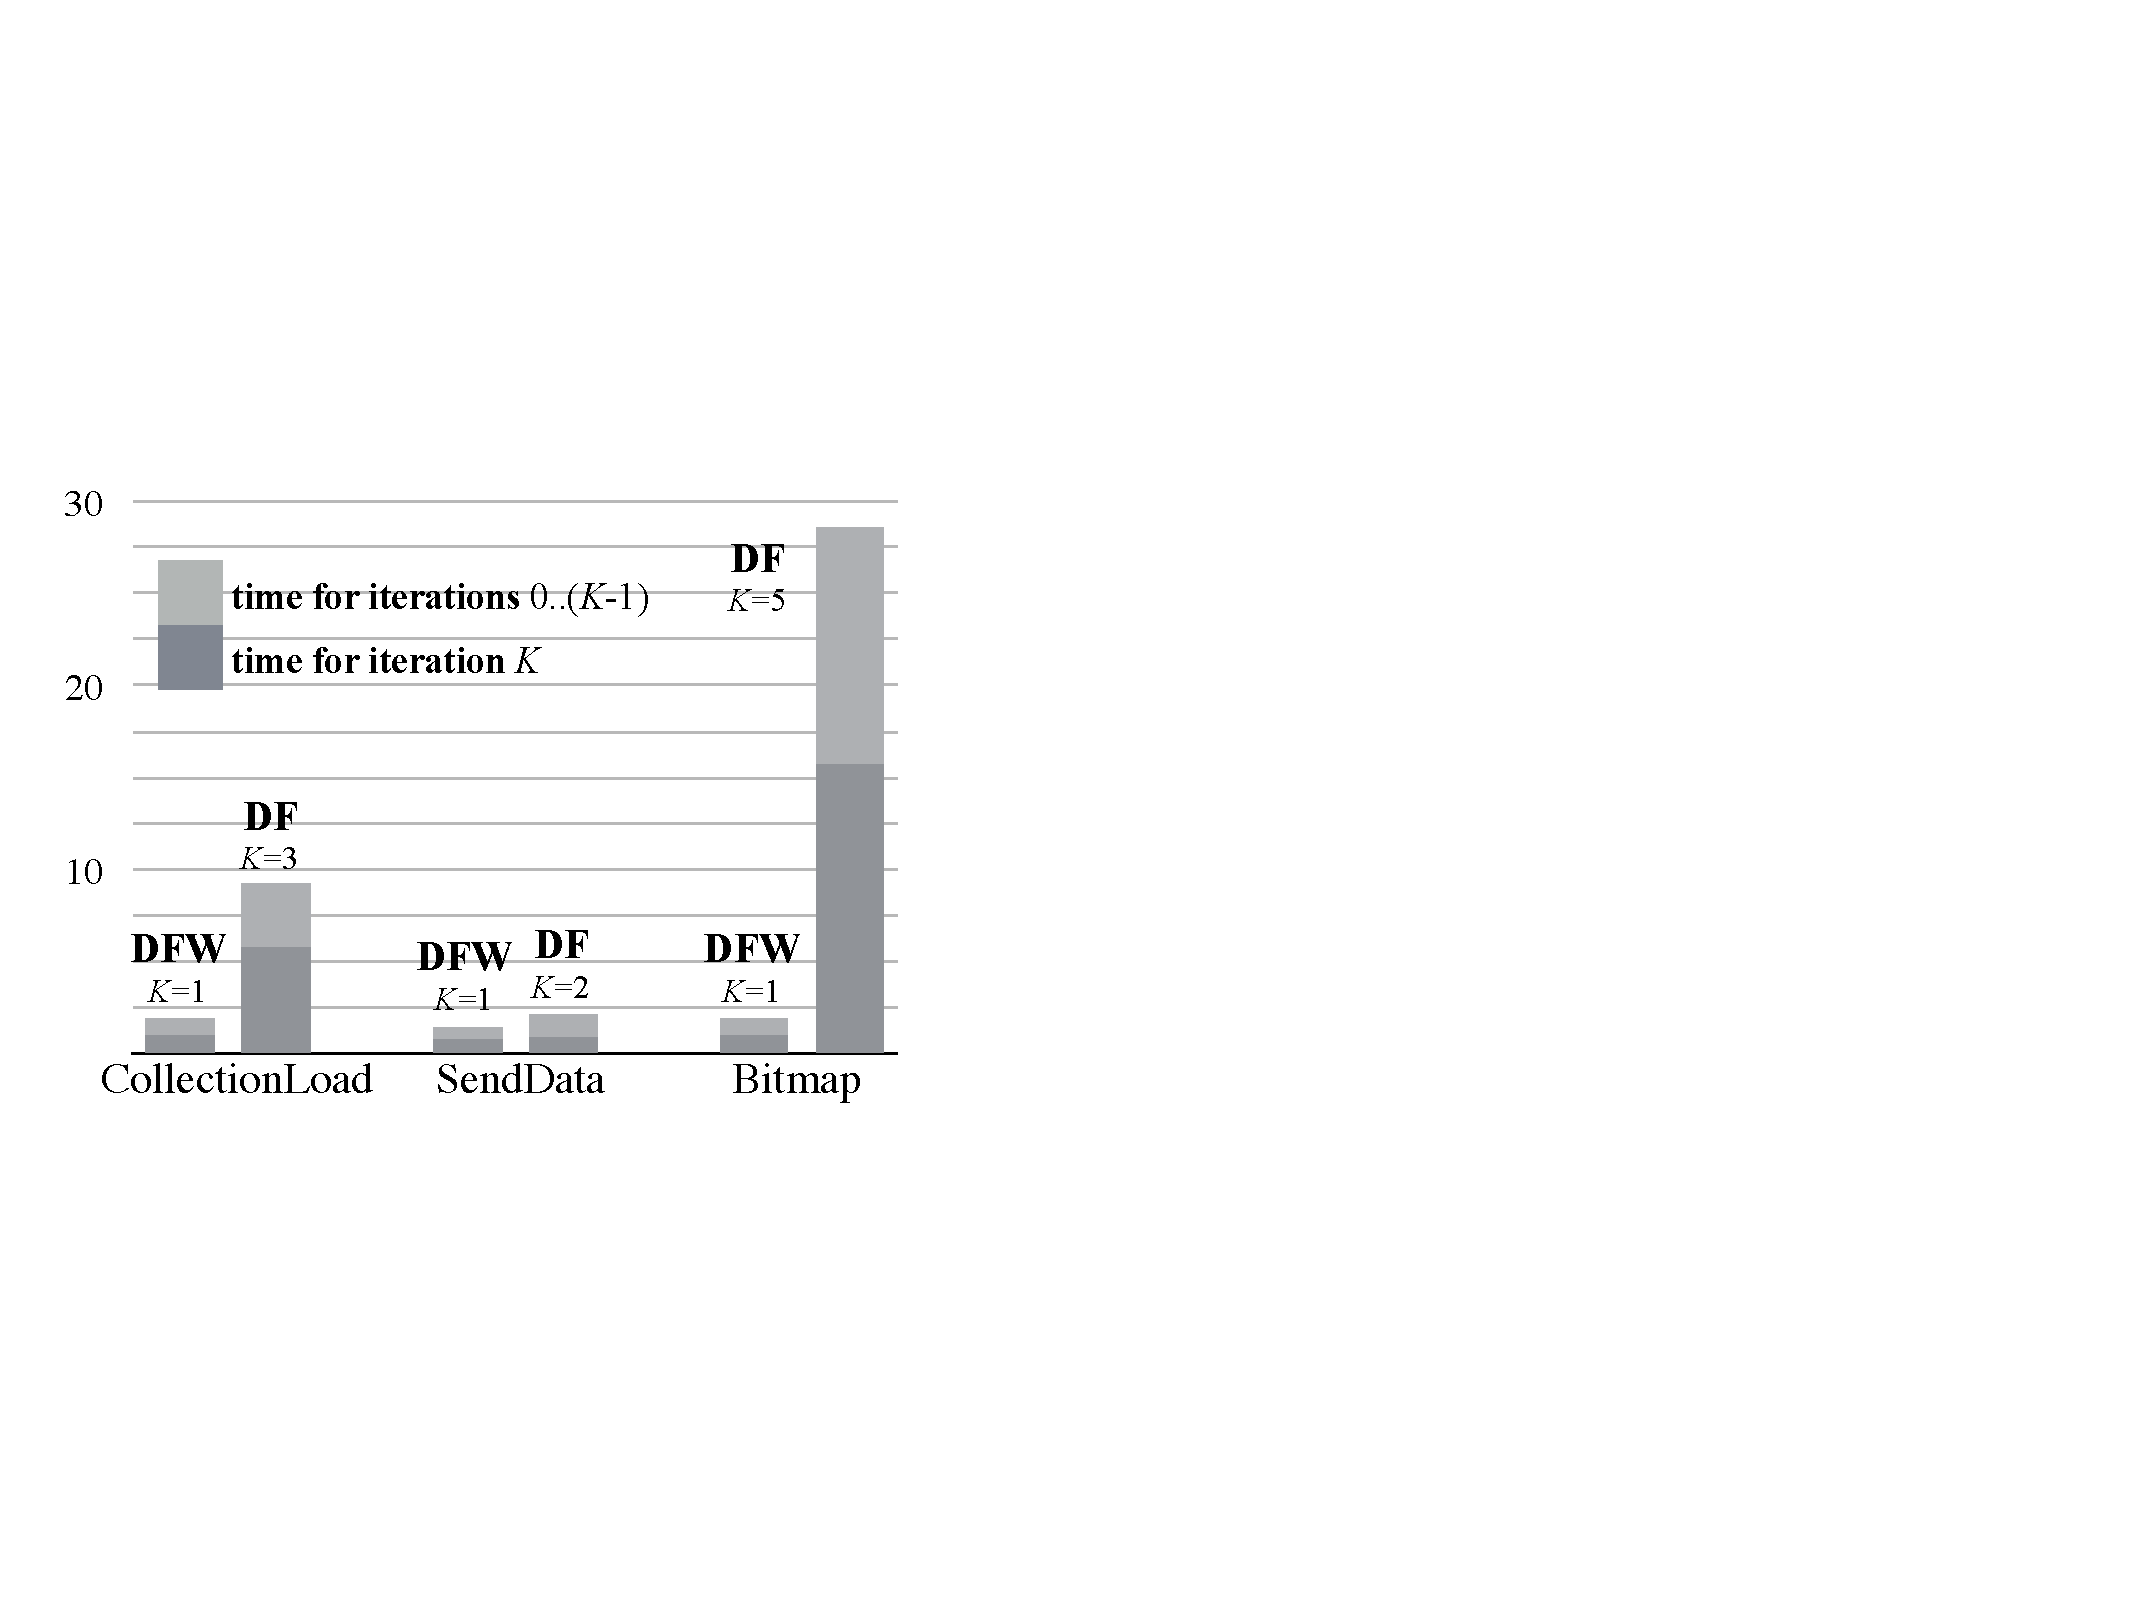
\includegraphics[width=6cm]{figures/figure-experiments-1}
  \caption{Time to bug detection (in seconds for three
    examples using the DFW and DF sequentializations.  Each bar represents 
    the aggregate time over increasing delay bounds, starting from zero,
    whereas the dark part indicates time spent for the smallest successful delay
    bound ($K$).
  }
  \label{fig:exp:csharp}
\end{figure}

\begin{figure}[t]
  \centering
  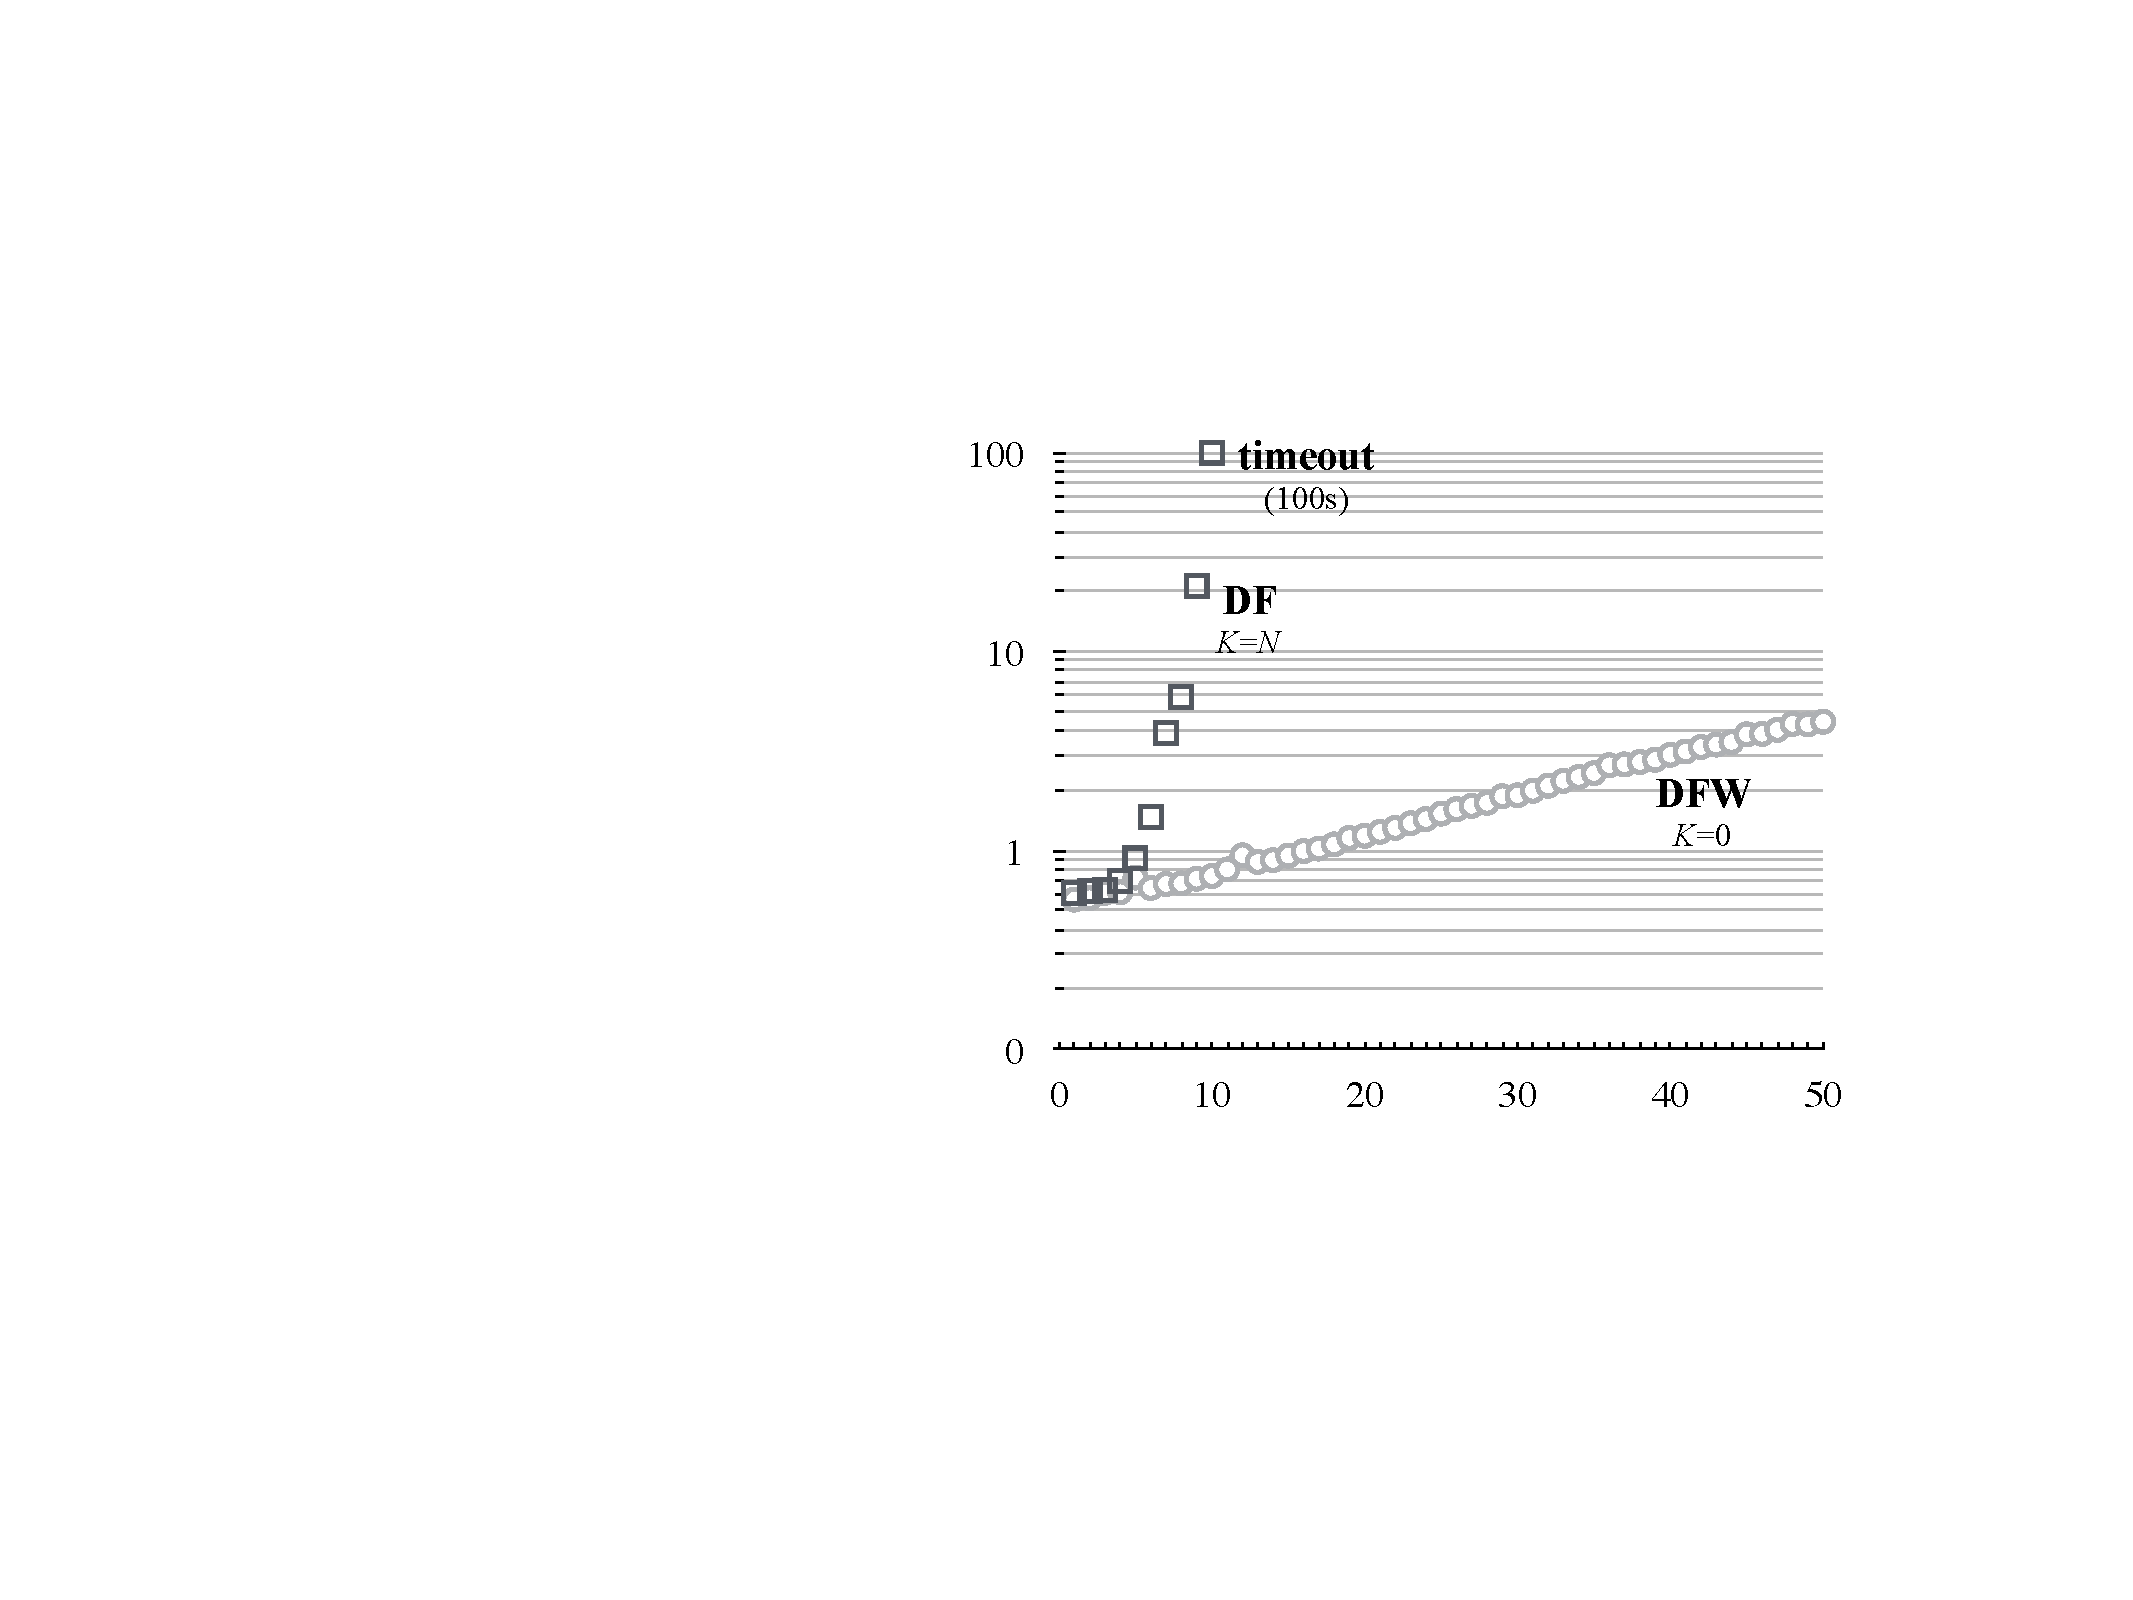
\includegraphics[width=6cm]{figures/figure-experiments-2}
  \caption{Time to bug detection (in seconds) for the
    parameterized example with $N$ (on the X-axis) chained asynchronous calls.
    While the DFW sequentialization consistently discovers the bug without
    delays, DF requires $K=N$ delays, and times out at 100s for $N=10$.}
  \label{fig:exp:param}
\end{figure}

In order to validate the efficacy of our delay-bounded sequentialization
approach, we have also implemented a ``depth-bounded'' exploration by
translating (by hand) the first {\tt CollectionLoad} example into a sequential
program which simulates every asynchronous program execution up to a given
number of program steps --- we consider that each program statement constitutes
one program step. This program's top-level procedure contains a loop in which
each iteration executes a single step of a nondeterministically-chosen task;
$K$ iterations of this top-level loop thus simulates all possible asynchronous
program executions with up to $K$ steps. Exploration of this program with
Corral is intractable: the same bug discovered with $\dfw(1)$ requires $K=9$
program steps, yet Corral is only able to explore up to $K=4$, in 90 seconds,
before timing out at 100 seconds for any depth $K\ge 5$. Note that while
$\dfw(K)$ is practically limited by the degree $K$ of deviation from $\dfw(0)$,
of which small values seem to suffice in exposing concurrency errors, $\dfw(K)$
is not inherently limited by execution depth.

Our second set of experiments attempts to measure the effect of the
aforementioned asynchronous call chains on the $\df(K)$ and
$\dfw(K)$ sequentializations using a very simple parameterized program
$P(N)$: for each $N \in \<Nats>$, $P(N)$ makes $N$ asynchronous calls (to a
procedure which simply returns) waiting for each before calling the next,
ultimately followed by an assertion violation ---
i.e.,~\lstinline{assert false}. As Figure~\ref{fig:exp:param} illustrates, the
$\dfw(K)$ scheduler never requires a delay to reach the assertion, and
its sequentialization scales well, with Corral completing in under 5 seconds
even for chains of 50 calls. The $\df(K)$ scheduler, however, requires
$N$ delays for each chain of $N$ calls, and times out at 100 seconds without
completing for chains of 10 calls. The utter simplicity of the program $P(N)$
suggests that the $\df(K)$ sequentialization is limited to very small
chains, and ultimately small fragments of synchronization-heavy programs.
